\let\negmedspace\undefined
\let\negthickspace\undefined
\documentclass[journal]{IEEEtran}
\usepackage[a5paper, margin=10mm, onecolumn]{geometry}
%\usepackage{lmodern} % Ensure lmodern is loaded for pdflatex
% \usepackage{tfrupee} % Include tfrupee package

\setlength{\headheight}{1cm} % Set the height of the header box
\setlength{\headsep}{0mm}     % Set the distance between the header box and the top of the text

\usepackage{gvv-book}
\usepackage{gvv}
\usepackage{cite}
\usepackage{amsmath,amssymb,amsfonts,amsthm}
\usepackage{algorithm}
\usepackage{algorithmic}
\usepackage{graphicx}
\usepackage{textcomp}
\usepackage{xcolor}
\usepackage{txfonts}
\usepackage{listings}
\usepackage{enumitem}
\usepackage{mathtools}
\usepackage{gensymb}
\usepackage{comment}
\usepackage[breaklinks=true]{hyperref}
\usepackage{tkz-euclide} 
\usepackage{listings}
% \usepackage{gvv}                                        
\def\inputGnumericTable{}                                 
\usepackage[latin1]{inputenc}                                
\usepackage{color}                                            
\usepackage{array}                                            
\usepackage{longtable}                
\usepackage{calc}                                             
\usepackage{multirow}                                         
\usepackage{hhline}                                           
\usepackage{ifthen}                             
\usepackage{caption}              
\usepackage{lscape}
\usepackage{subcaption}
\usepackage{circuitikz}
\captionsetup{compatibility=false}
% \captionsetup{compactibility=false}
% \usepackage{algpseudocode}
\begin{document}

\bibliographystyle{IEEEtran}
\vspace{3cm}

\title{Experiment 4} 
\author{S A Aravind Eswar and Eshan Sharma}
{\let\newpage\relax\maketitle}

\section{Aim}

To study and analyze the transient response of an LC circuit, determine the natural frequency (\(\Omega_n\)), and calculate the damping ratio (\(\xi\)) using theoretical and experimental methods.

\section{Materials and Apparatus Required}

\begin{enumerate}
	\item 100 $\mu$F Capacitor
	\item Largest available inductor in the lab (denoted as \(L\))
	\item Resistor (small value for practical considerations)
	\item DC Power Supply
	\item Oscilloscope
\end{enumerate}

\section{Theory}

An LC circuit consists of an inductor (\(L\)) and a capacitor (\(C\)) connected in parallel. When a charged capacitor is connected to an inductor, energy oscillates between the capacitor's electric field and the inductor's magnetic field. This oscillatory behavior is governed by the second-order differential equation:
\[
L \frac{d^2q}{dt^2} + \frac{q}{C} = 0,
\]
where \(q(t)\) is the charge on the capacitor as a function of time.

The natural frequency of oscillation is given by:
\[
\Omega_n = \frac{1}{\sqrt{LC}},
\]
where:
- \(L\) is the inductance in henries (H),
- \(C\) is the capacitance in farads (F).

For an ideal LC circuit (no resistance), the damping ratio (\(\xi = 0\)) indicates purely oscillatory behavior. However, in practical circuits, resistance (\(R\)) introduces damping, and the damping ratio becomes:
\[
\xi = \frac{R}{2} \sqrt{\frac{C}{L}}.
\]

\subsection{Theoretical Calculations for Given Values}
Given:
\begin{itemize}
	\item Capacitance, \(C = 1 \, \text{nF} = 1 \times 10^{-9} \, \text{F}\),
	\item Inductance, \(L = 2.2 \, \text{mH} = 2.2 \times 10^{-3} \, \text{H}\),
	\item Internal resistance of the inductor, \(R = 25.2 \, \Omega\).
\end{itemize}

\subsubsection{Natural Frequency (\(\Omega_n\))}
\[
\Omega_n = \frac{1}{\sqrt{LC}} = \frac{1}{\sqrt{(2.2 \times 10^{-3}) (1 \times 10^{-9})}}.
\]
Simplifying:
\[
\Omega_n = \frac{1}{\sqrt{2.2 \times 10^{-12}}} = \frac{1}{1.483 \times 10^{-6}}} \approx 6.74 \times 10^5 \, \text{rad/s}.
\]

\subsubsection{Damping Ratio (\(\xi\))}
\[
\xi = \frac{R}{2} \sqrt{\frac{C}{L}} = \frac{25.2}{2} \sqrt{\frac{1 \times 10^{-9}}{2.2 \times 10^{-3}}}.
\]
Simplifying:
\[
\xi = 12.6 \sqrt{\frac{10^{-9}}{2.2 \times 10^{-3}}} = 12.6 \sqrt{4.545 \times 10^{-7}}}.
\]
Further simplification:
\[
\xi = 12.6 \times 6.74 \times 10^{-4} \approx 0.0085.
\]

Since \(\xi \approx 0.0085\), which is much less than 1, the circuit is \textbf{underdamped}, and oscillations will decay over time.

---

The transient response of the LC circuit can be classified based on the value of \(\xi\):
\begin{enumerate}
\item \textbf{Underdamped (\(0 < \xi < 1\)):} Oscillations decay over time.
\item \textbf{Critically damped (\(\xi = 1\)):} Fastest return to equilibrium without oscillation.
\item \textbf{Overdamped (\(\xi > 1\)):} Slow return to equilibrium without oscillation.
\end{enumerate}

The voltage across the capacitor during oscillations can be expressed as:
\[
V_C(t) = V_0 e^{-\xi \Omega_n t} \cos(\Omega_d t + \phi),
\]
where:
\begin{itemize}
\item \(V_0\) is the initial voltage,
\item \(\Omega_d = \Omega_n \sqrt{1 - \xi^2}\) is the damped natural frequency,
\item \(\phi\) is the phase angle.
\end{itemize}

\begin{figure}[!ht]
	\centering
	\resizebox{0.6\textwidth}{!}{
		\begin{circuitikz}
			\tikzstyle{every node}=[font=\LARGE]
			\draw (10.5,13) to[R] (10.5,11.25);
			\draw (12.25,14) to[L ] (14.25,14);
			\draw (15.75,13) to[C] (15.75,11.25);
			\draw (10.5,13) to[short] (10.5,14);
			\draw (10.5,14) to[short] (12.25,14);
			\draw (14.25,14) to[short] (15.75,14);
			\draw (15.75,14) to[short] (15.75,13);
			\draw (10.5,10.25) to[short] (15.75,10.25);
			\draw (15.75,11.25) to[short] (15.75,10.25);
			\draw (10.5,11.25) to[short] (10.5,10.25);
			\node [font=\LARGE] at (11,11.5) {$+$};
			\node [font=\LARGE] at (12.5,14.25) {$+$};
			\node [font=\LARGE] at (15.5,11.5) {$+$};
			\node [font=\LARGE] at (14,14.25) {$-$};
			\node [font=\LARGE] at (15.5,12.75) {$-$};
			\node [font=\LARGE] at (11,12.75) {$-$};
			\draw [->, >=Stealth] (12.5,11.75) .. controls (12.25,12.75) and (14,13) .. (13.75,11.75) ;
			\node [font=\LARGE] at (13,11.75) {i};
		\end{circuitikz}
	}
	\label{fig:LC circuit with internal resistance}
	
\end{figure}


For experimental analysis, we monitor voltage waveforms using an oscilloscope. The observed oscillation frequency can be compared with theoretical calculations to validate the model.

In summary:
\begin{itemize}
	\item For a purely LC circuit: \(R = 0, \xi = 0, \Omega_d = \Omega_n.\)
	\item For an RLC circuit: \(R > 0,\) leading to damping and reduced oscillation frequency.
\end{itemize}

The energy exchange between components can be calculated as:
\begin{itemize}
	\item Energy stored in capacitor: \(E_C = \frac{1}{2} C V_C^2,\)
	\item Energy stored in inductor: \(E_L = \frac{1}{2} L I^2,\) where \(I = -C \frac{dV_C}{dt}.\)
\end{itemize}

These equations form the basis for analyzing transient responses.

\section{Procedure}

\begin{enumerate}
	\item Precharge the Capacitor:
	\begin{itemize}
		\item Connect the 100 $\mu$F capacitor to a 5V DC power supply.
		\item Once charged, disconnect it carefully without discharging.
	\end{itemize}
	
	\item Construct the LC Circuit:
	\begin{itemize}
		\item Connect the charged capacitor in parallel with the largest available inductor.
		\item Ensure minimal resistance in wiring.
	\end{itemize}
	
	\item Capture Transient Response:
	\begin{itemize}
		\item Use an oscilloscope to monitor voltage across the capacitor.
		\item Observe natural oscillations.
	\end{itemize}
	
	\item Calculate Theoretical Values:
	\begin{itemize}
		\item Compute natural frequency (\(\Omega_n = 1/\sqrt{LC}\)).
		\item Estimate damping ratio (\(\xi = R/2\sqrt{\frac{C}{L}}\)) if resistance is non-negligible.
	\end{itemize}
	
	\item Compare with Experimental Results:
	\begin{itemize}
		\item Extract oscillation frequency from oscilloscope data.
		\item Compare with theoretical calculations.
	\end{itemize}

	
\end{enumerate}

\section{Observations}

\begin{figure}[h]
	\centering
	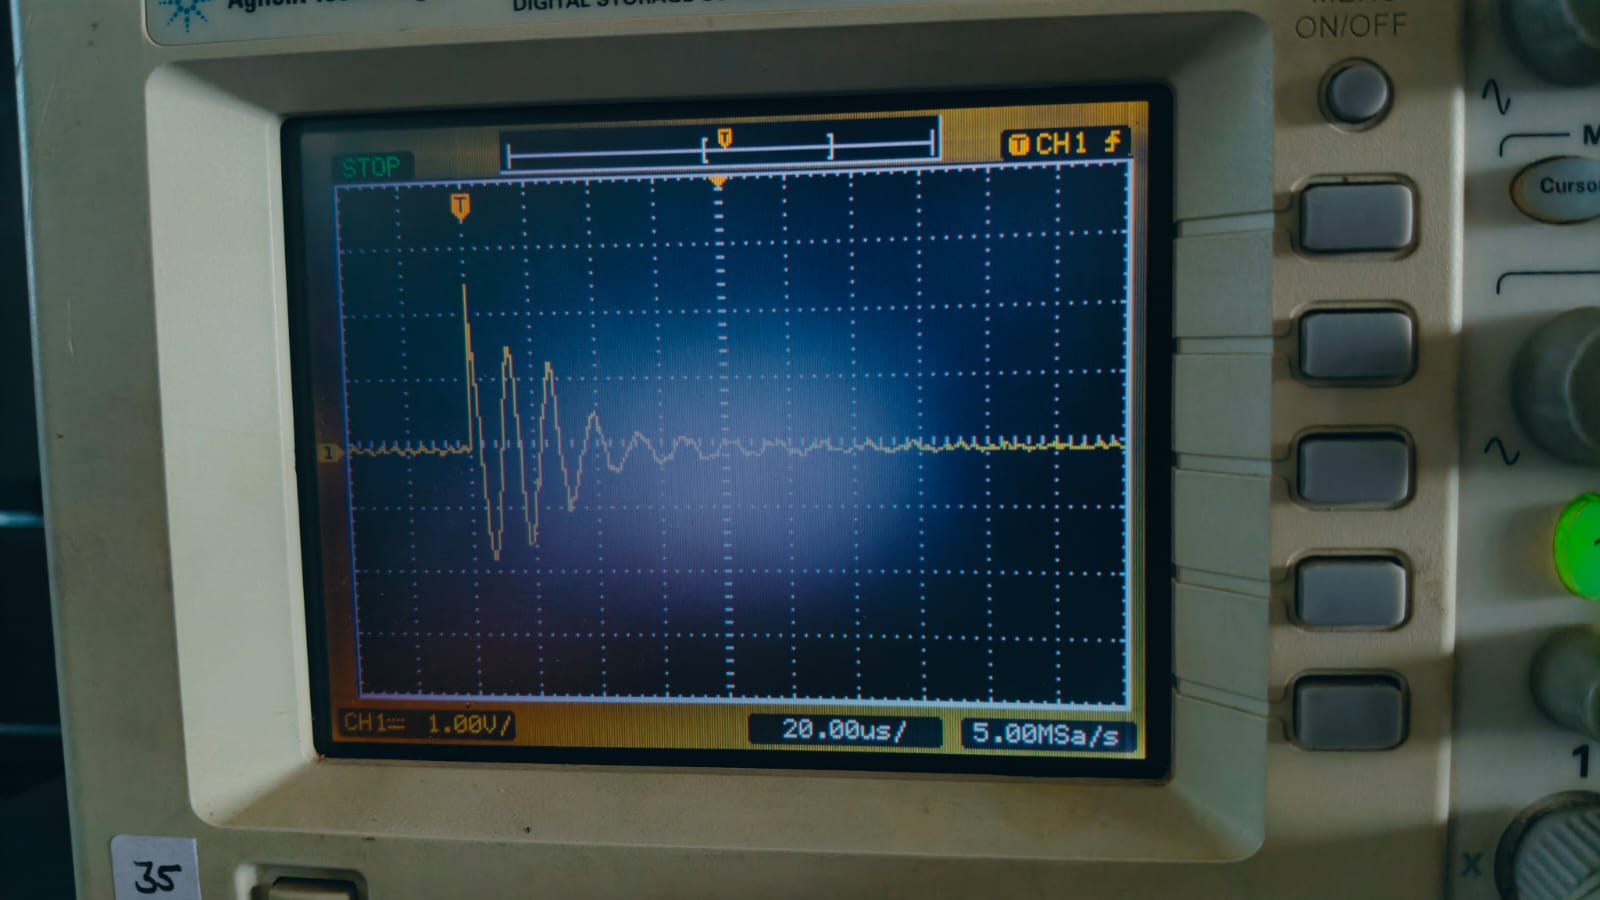
\includegraphics[width=0.7\columnwidth]{figs/LC.jpeg}
	\caption{Transient Response of LC}
\end{figure}

\end{document}
